\documentclass[tikz]{standalone}
\usepackage{pgfplots}
\pgfplotsset{compat=1.15}
\usepackage{mathrsfs}
\usetikzlibrary{arrows,calc}
\usepackage{tkz-euclide}
\pagestyle{empty}

\definecolor{AngleClr}{rgb}{0,0.39215686274509803,0}
\definecolor{ShapeClr}{rgb}{0.6,0.2,0}

\begin{document}

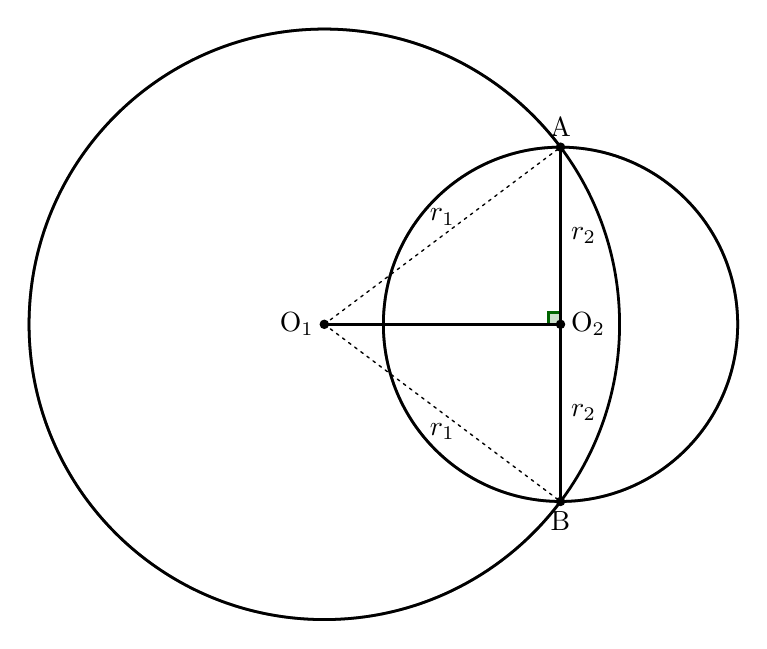
\begin{tikzpicture}[scale=.75]
\tkzSetUpLine[line width=1pt,color=black]
\tkzSetUpPoint[fill=black]

\tkzDefPoints{0/0/O1,4/0/O2,5/0/A,7/0/B}


\tkzDrawCircle[line width=1.0pt,fill=white](O1,A)
\tkzDrawCircle[line width=1.0pt,fill=white](O2,B)

\tkzDrawCircle[line width=1.0pt,color=black](O1,A)
\tkzDrawCircle[line width=1.0pt,color=black](O2,B)

\tkzInterCC(O1,A)(O2,B) \tkzGetPoints{C}{D}
\tkzInterLL(O1,O2)(C,D) \tkzGetPoint{I}
\tkzMarkRightAngles[line width=1pt, size=.2,color=AngleClr,fill=AngleClr,fill opacity=0.2](C,I,O1)

\tkzDrawSegments[line width=1pt,color=black](C,D O1,O2)
\tkzDrawSegments[line width=0.5pt,color=black,dashed,dash pattern=on 1pt off 1.75pt](O1,C O1,D)


\tkzDrawPoints[size=3](O1,O2,C,D)
\tkzLabelPoint[left](O1){$\rm O_1$}
\tkzLabelPoint[right](O2){$\rm O_2$}
\tkzLabelPoint[above](C){$\rm A$}
\tkzLabelPoint[below](D){$\rm B$}
\tkzLabelSegment[above](O1,C){$r_1$}
\tkzLabelSegment[below](O1,D){$r_1$}
\tkzLabelSegment[right](O2,C){$r_2$}
\tkzLabelSegment[right](O2,D){$r_2$}

\end{tikzpicture}
\end{document}
